
\documentclass{article}

\usepackage{graphicx}
\usepackage{geometry}
\geometry{a4paper}
\setlength{\lineskip}{3.5pt}
\setlength{\lineskiplimit}{200pt}
\setlength{\baselineskip}{100pt}

\begin{document}
\linespread{2}
\begin{center}
 	{\Huge Proyecto - Sección 1.2}\\
	 \vspace{0.75cm}
	 {\large Probabilidad y Estadística ejercicios}\\
	 \vspace{0.5cm}
 	{\large Daniela Jijón, Juan Francisco Cisneros y Luciana Valdivieso}\\
	\vspace{0.5cm}
 	{\large 18 de junio de 2022}\\
	\vspace{0.5cm}
 	\line(1,0){375}
	\vspace{0.5cm}
\end{center}
	
\section*{Estadísticas Descriptivas}
\subsection*{Cálculos}
Los cálculos se realizaron con Excel y Python.\\El tamaño de la muestra de los datos recolectados es n=202. 
\subsubsection*{Media}
La media representa el valor promedio de los datos, se representa como la sumatoria de todos los datos dividido para el numero de datos n. La sumatoria de los n valores se realiza iterando por cada valor de la variable y sumándolos.
\begin{center}
	\=x $= \frac{\sum_{i=1}^n x_{i}}{n}$\\
\end{center}
Edad: \\                                           \=x $= \frac{\sum_{i=1}^{202}  x_{i}}{202} = 19.7$ ,  20 años \vspace{0.25cm} \\
Año de estudio:\\                           \=x $=\frac{\sum_{i=1}^{202}  x_{i}}{202} =  2.3$ ,   segundo año de carrera \vspace{0.25cm}\\
Horas de estudio por semana:\\      \=x $= \frac{\sum_{i=1}^{202}  x_{i}}{202} = 12.2$ \vspace{0.25cm}\\
GPA ponderado:\\                         \=x $= \frac{\sum_{i=1}^{202}  x_{i}}{202} =  3.47 $ \vspace{0.25cm}\\

\subsubsection*{Mediana}
Para calcular el valor de la mediana necesitamos la posición del valor. Los valores deben estar ordenados de menor a mayor, en el codigo se transfieren los n valores de cada variabe a una lista para poder ser ordenados y acceder a la posición del valor de la media. Dado que n es par, por lo que se usa la formula que es el promedio entre  $(\frac{n}{2})^{n-esima}$ y
$(\frac{n}{2} + 1)^{n-esima}$ posición. \\
\begin{center}
	$(\frac{202}{2})^{n-esima} + (\frac{202}{2} + 1)^{n-esima} = 203$\\
	$\frac{203}{2} = 101.5^{n-esima}$ posición\\
\end{center}
Edad:\\                                           \~x $= 19$ \vspace{0.25cm}\\
Año de estudio:\\                             \~x $= 2 $ \vspace{0.25cm}\\
Horas de estudio por semana:\\      \~x $=13 $ \vspace{0.25cm}\\
GPA ponderado:\\                           \~x $=  3.5$ \vspace{0.25cm}\\

\subsubsection*{Moda}
La moda es el valor más frecuente.\vspace{0.25cm}\\
Edad:\\                                            Mo $= 18$ \vspace{0.25cm}\\
Año de estudio:\\                            Mo $= 2$\vspace{0.25cm}\\
Horas de estudio por semana:\\      Mo $=  8$\vspace{0.25cm}\\
GPA ponderado:\\                            Mo $=  4$\vspace{0.25cm}\\

\subsubsection*{Varianza y Desviación Estandar}
\begin{center}
	$s^{2}  = \frac{\sum_{i=1}^n (x_{i}-\=x)^{2}}{n-1}$\\
	$s^{2}  = \frac{\sum_{i=1}^{202} (x_{i}-\=x)^{2}}{202-1}$\\
	$s = \sqrt[2]{s^{2}}$\\
\end{center}
Edad:\\                                          $s^{2} = \frac{\sum_{i=1}^{202} (x_{i}-19.7)^{2}}{202-1} = 3.4 $\\$s = 1.98$\vspace{0.25cm}\\
Año de estudio: \\                          $s^{2} =   \frac{\sum_{i=1}^{202} (x_{i}-2.3)^{2}}{202-1} =1.35$\\$s = 1.21 $\vspace{0.25cm}\\
Horas de estudio por semana:\\    $s^{2} =  \frac{\sum_{i=1}^{202} (x_{i}-12.2)^{2}}{202-1} = 49.28$\\$s = 7.06$\vspace{0.25cm}\\
GPA ponderado:\\                          $s^{2} =  \frac{\sum_{i=1}^{202} (x_{i}-3.47)^{2}}{202-1} = 0.16$\\$s = 0.4$\vspace{0.25cm}\\

\subsubsection*{Cuartiles}
Para los cuartiles debemos usar la fórmula de percentiles, son los percentiles 25, 50, 75 y 100.\\
$i = \frac{25}{100}(n+1)=50.5$ \\
$i = \frac{50}{100}(n+1)=101$ \\
$i = \frac{75}{100}(n+1)= 151.5$\vspace{0.25cm}\\
Para las posiciones no enteras, se deben promediar las posiciones i e i+1\\
Edad:\\                                          $Q_{1}= 18$\\$Q_{2}=19$\\$Q_{3}=20$\vspace{0.25cm}\\
Año de estudio: \\                          $Q_{1}= 1$\\$Q_{2}=2$\\$Q_{3}=3$\vspace{0.25cm}\\
Horas de estudio por semana:\\    $Q_{1}= 8$\\$Q_{2}=13$\\$Q_{3}=18$\vspace{0.25cm}\\
GPA ponderado:\\                          $Q_{1}= 3.2$\\$Q_{2}=3.5$\\$Q_{3}=3.8$\vspace{0.25cm}\\

\subsubsection*{Rango Intercuartil}
Usamos los valores obtenidos para los cuartiles y reemplazamos en la fórmula del rango intercuartil (Ric), este valor resultante indica la distancia entre el primer y tercer cuartil.\par
\begin{center}
$Ric = Q_{3}-Q_{1}$\\
\end{center}
Edad:\\                                          $Ric = 20-18 = 2$\vspace{0.25cm}\\
Año de estudio: \\                          $Ric = 3-1 = 2$\vspace{0.25cm}\\
Horas de estudio por semana:\\    $Ric = 18-8 = 10$\vspace{0.25cm}\\
GPA ponderado:\\                          $Ric = 3.8-3.2 = 0.6$\vspace{0.25cm}\\

\subsubsection*{Percentil 10}
\begin{center}
$i = \frac{k}{100}(n)$\\
$i = \frac{10}{100}(202) = 20,3$\\
\end{center}
Ya que el valor de i no es entero, la posición del percentil es el entero inmediato superior, posición 21 de los ordenados.\vspace{0.25cm}\\
Edad:\\                                          $P_{10}= 18$\vspace{0.25cm}\\
Año de estudio: \\                          $P_{10}= 1$\vspace{0.25cm}\\
Horas de estudio por semana:\\    $P_{10}= 2.5$\vspace{0.25cm}\\
GPA ponderado:\\                          $P_{10}= 3$\vspace{0.25cm}\\
\subsubsection*{Limites superior e inferior}
Para calcular los límites superiores e inferiores debemos ordenar nuestros datos de menor a mayor. Una vez ordenados tomamos como límite inferior el valor más pequeño y cómo superior el valor más alto.\vspace{0.25cm}\\

\subsection*{Gráficos}
\subsubsection*{Variables Cuantitativas}
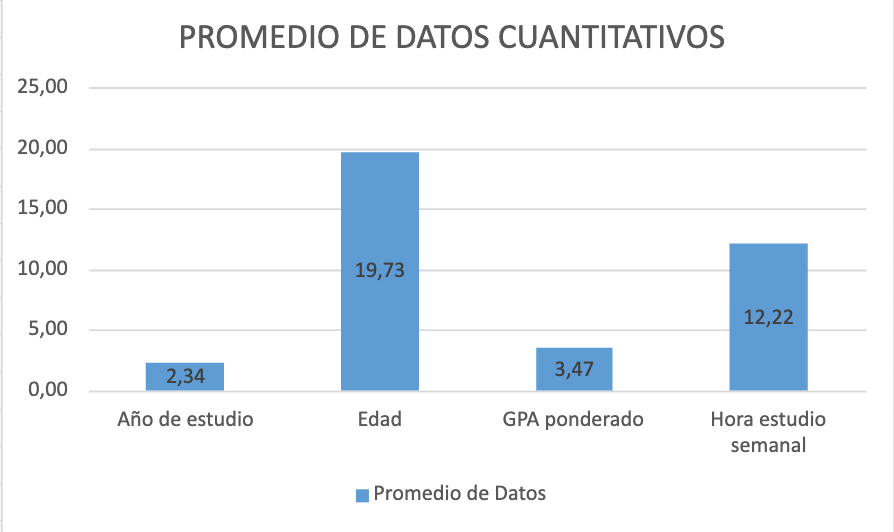
\includegraphics[width=8cm, height=7cm]{histo}
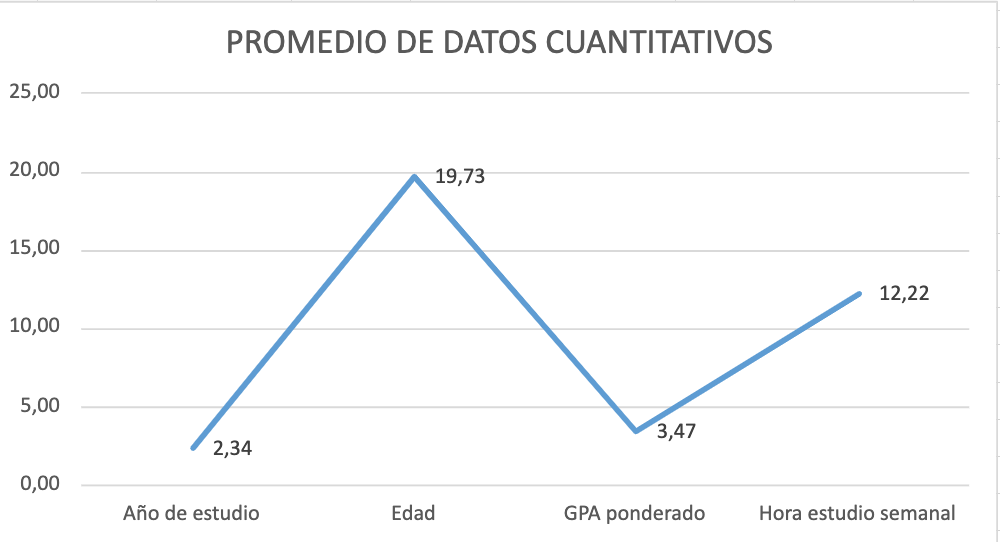
\includegraphics[width=8cm, height=7cm]{poligono}\vspace{0.25cm}\\

Box Plots comparativos:\vspace{0.25cm}\\
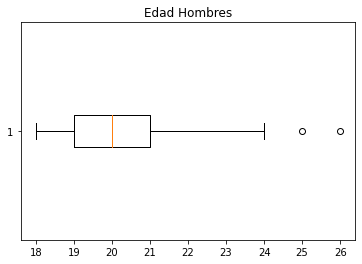
\includegraphics[width=8cm, height=7cm]{Edad_hombres}
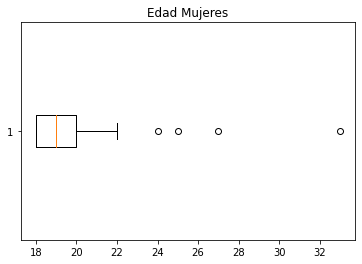
\includegraphics[width=8cm, height=7cm]{Edad_mujeres}
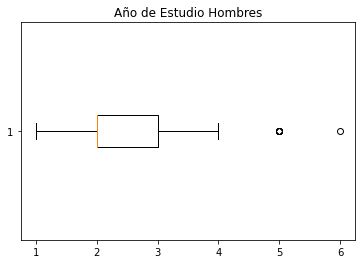
\includegraphics[width=8cm, height=7cm]{Year_hombres}
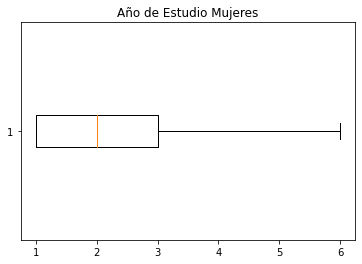
\includegraphics[width=8cm, height=7cm]{Year_mujeres}
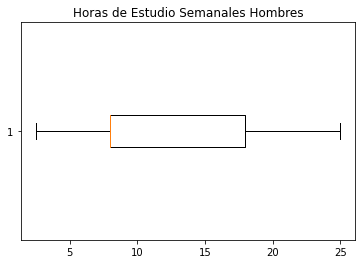
\includegraphics[width=8cm, height=7cm]{Horas_hombres}
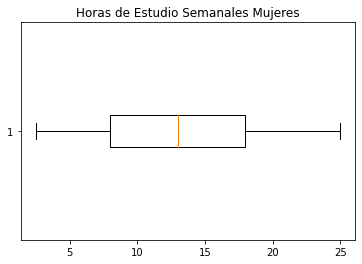
\includegraphics[width=8cm, height=7cm]{Horas_mujeres}
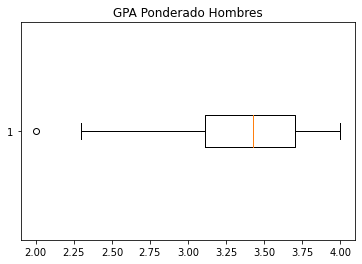
\includegraphics[width=8cm, height=7cm]{GPA_hombres}
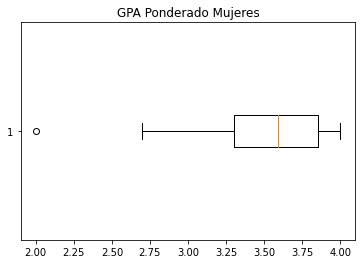
\includegraphics[width=8cm, height=7cm]{GPA_mujeres}

\subsubsection*{Variables Cualitativas}
Pie charts comparativos:\\
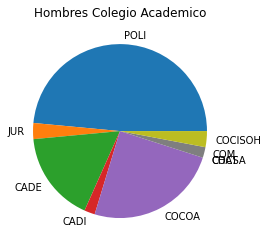
\includegraphics[width=8cm, height=7cm]{Colegio_hombres}
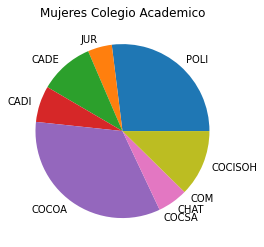
\includegraphics[width=8cm, height=7cm]{Colegio_mujeres}
\includegraphics[width=8cm, height=7cm]{Pie_sexo}\vspace{1cm}\\
Bar charts comparativos:\\
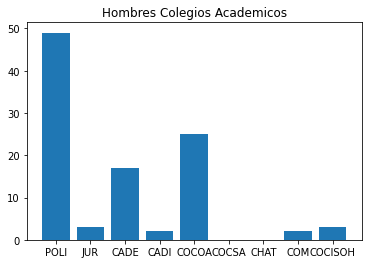
\includegraphics[width=8cm, height=7cm]{bar_colegios_hombres}
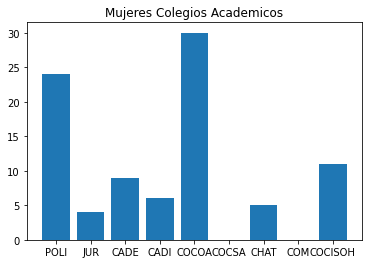
\includegraphics[width=8cm, height=7cm]{bar_colegios_mujeres}


\end{document}